
% !TEX option = -shell-escape
\documentclass[a4paper,UKenglish,cleveref, autoref, thm-restate, anonymous]{lipics-v2021}
%This is a template for producing LIPIcs articles. 
%See lipics-v2021-authors-guidelines.pdf for further information.
%for A4 paper format use option "a4paper", for US-letter use option "letterpaper"
%for british hyphenation rules use option "UKenglish", for american hyphenation rules use option "USenglish"
%for section-numbered lemmas etc., use "numberwithinsect"
%for enabling cleveref support, use "cleveref"
%for enabling autoref support, use "autoref"
%for anonymousing the authors (e.g. for double-blind review), add "anonymous"
%for enabling thm-restate support, use "thm-restate"
%for enabling a two-column layout for the author/affilation part (only applicable for > 6 authors), use "authorcolumns"
%for producing a PDF according the PDF/A standard, add "pdfa"

%\pdfoutput=1 %uncomment to ensure pdflatex processing (mandatatory e.g. to submit to arXiv)
%\hideLIPIcs  %uncomment to remove references to LIPIcs series (logo, DOI, ...), e.g. when preparing a pre-final version to be uploaded to arXiv or another public repository

%\graphicspath{{./graphics/}}%helpful if your graphic files are in another directory

\usepackage{algorithm}
\usepackage{graphicx}
\usepackage{amsmath}
\usepackage{listings}
\usepackage{array}
\usepackage{bm}
\usepackage{hyperref}
\usepackage{todonotes}
\usepackage{subcaption}
\usepackage{colortbl}
\usepackage{censor}
\usepackage{wrapfig}    
\usepackage{listings}
\usepackage{xcolor}
\definecolor{lightgray}{rgb}{0.95,0.95,0.95}
\lstdefinelanguage{Coq}{
  keywords={Definition,Inductive,Fixpoint,Theorem,Lemma,Proof,Qed,End,Section,match,with,end,fun,forall,if,then,else,let,in,where,as,return,Set,Prop,Type},
  sensitive=true,
  morecomment=[n]{(*}{*)},
  morestring=[b]{"},
}
\lstset{
  basicstyle=\footnotesize\ttfamily,
  backgroundcolor=\color{lightgray},
  frame=single,
  breaklines=true,
  showstringspaces=false,
}
\usepackage{mathpartir}
\usepackage[most]{tcolorbox}
\usetikzlibrary{arrows}
\usepackage{float}
\usepackage{bclogo}
\setlength{\parindent}{0pt}



\bibliographystyle{plainurl}% the mandatory bibstyle

\title{Verified Fixed-Point Computation over Bounded Semirings\\with Applications to Voting and Optimisation} %TODO Please add


\author{Jane {Open Access}}{Dummy University Computing Laboratory, [optional: Address], Country \and My second affiliation, Country \and \url{http://www.myhomepage.edu} }{johnqpublic@dummyuni.org}{https://orcid.org/0000-0002-1825-0097}{(Optional) author-specific funding acknowledgements}%TODO mandatory, please use full name; only 1 author per \author macro; first two parameters are mandatory, other parameters can be empty. Please provide at least the name of the affiliation and the country. The full address is optional. Use additional curly braces to indicate the correct name splitting when the last name consists of multiple name parts.


%\author{{Mukesh Tiwari\inst{1}\orcidID{0000-0001-5373-9659}} \and
%{Nobuko Yoshida \inst{2}\orcidID{0000-0002-3925-8557}} \and
%{Mina A. Cyrus\inst{1}\orcidID{0009-0005-9085-4652}}}
%
%\authorrunning{Mukesh Tiwari, Nobuko Yoshida, and Mina Cyrus}
% First names are abbreviated in the running head.
% If there are more than two authors, 'et al.' is used.
%
%\institute{School of Mathematics and Computer Science, Swansea University, UK
%\email{\{mukesh.tiwari, m.a.cyrus\}@swansea.ac.uk} \and
%Department of Computer Science, University of Oxford, UK\\
%\email{nobuko.yoshida@cs.ox.ac.uk}
%}
%
\Copyright{CC-BY} %TODO mandatory, please use full first names. LIPIcs license is "CC-BY";  http://creativecommons.org/licenses/by/3.0/

\begin{CCSXML}
<ccs2012>
   <concept>
       <concept_id>10003752.10003790.10002990</concept_id>
       <concept_desc>Theory of computation~Logic and verification</concept_desc>
       <concept_significance>500</concept_significance>
       </concept>
   <concept>
       <concept_id>10003752.10003790.10003796</concept_id>
       <concept_desc>Theory of computation~Constructive mathematics</concept_desc>
       <concept_significance>500</concept_significance>
       </concept>
 </ccs2012>
\end{CCSXML}

\ccsdesc[500]{Theory of computation~Logic and verification}
\ccsdesc[500]{Theory of computation~Constructive mathematics}

%\ccsdesc[100]{\textcolor{red}{Replace ccsdesc macro with valid one}} %TODO mandatory: Please choose ACM 2012 classifications from https://dl.acm.org/ccs/ccs_flat.cfm 

\keywords{Semiring, Kleene Star, Fixed Point, Formal Verification, Coq, Voting, Optimisation, Semimodule} %TODO mandatory; please add comma-separated list of keywords

\category{} %optional, e.g. invited paper

%\relatedversion{} %optional, e.g. full version hosted on arXiv, HAL, or other respository/website
%\relatedversiondetails[linktext={opt. text shown instead of the URL}, cite=DBLP:books/mk/GrayR93]{Classification (e.g. Full Version, Extended Version, Previous Version}{URL to related version} %linktext and cite are optional

%\supplement{}%optional, e.g. related research data, source code, ... hosted on a repository like zenodo, figshare, GitHub, ...
%\supplementdetails[linktext={opt. text shown instead of the URL}, cite=DBLP:books/mk/GrayR93, subcategory={Description, Subcategory}, swhid={Software Heritage Identifier}]{General Classification (e.g. Software, Dataset, Model, ...)}{URL to related version} %linktext, cite, and subcategory are optional

%\funding{(Optional) general funding statement \dots}%optional, to capture a funding statement, which applies to all authors. Please enter author specific funding statements as fifth argument of the \author macro.

%\acknowledgements{I want to thank \dots}%optional

%\nolinenumbers %uncomment to disable line numbering



%Editor-only macros:: begin (do not touch as author)%%%%%%%%%%%%%%%%%%%%%%%%%%%%%%%%%%
\EventEditors{John Q. Open and Joan R. Access}
\EventNoEds{2}
\EventLongTitle{42nd Conference on Very Important Topics (CVIT 2016)}
\EventShortTitle{CVIT 2016}
\EventAcronym{CVIT}
\EventYear{2016}
\EventDate{December 24--27, 2016}
\EventLocation{Little Whinging, United Kingdom}
\EventLogo{}
\SeriesVolume{42}
\ArticleNo{23}
%%%%%%%%%%%%%%%%%%%%%%%%%%%%%%%%%%%%%%%%%%%%%%%%%%%%%%

\begin{document}
\nolinenumbers

\maketitle

%TODO mandatory: add short abstract of the document
\begin{abstract}
We present the first mechanically verified framework for computing fixed points (Kleene star) 
in bounded semirings, formalised in the Coq theorem prover. Our central result establishes 
that the formal power series $A^*$ of any $n \times n$ matrix over a bounded semiring 
converges after exactly $n-1$ iterations: $A^* = A^{\langle n - 1 \rangle}$. This unifies 
a wide class of graph algorithms---including shortest path, widest path, most reliable path, 
and the Schulze voting method---under a single algebraic abstraction. 

We demonstrate the generality of our framework through four verified instances: 
(i) the Schulze preferential voting method, which we validate against examples from Wikipedia 
and the original paper; (ii) the widest-shortest path optimisation problem; 
(iii) the Viterbi most-reliable-path semiring over rational probabilities; and 
(iv) a semimodule extension enabling linear equations $Ax = b$ over semirings, 
with applications to algebraic program analysis. Each instance requires only 
the instantiation of semiring operators and a proof of boundedness; 
the fixed-point computation and OCaml extraction follow automatically from the framework.
\end{abstract}


\section{Introduction}
Graph algorithms are among the most fundamental computational
problems in computer science. Algorithms for shortest paths
\cite{10.1007/BF01386390}, maximum flow \cite{ford_fulkerson_1956},
transitive closure \cite{abdali1985transitive}, and many others
appear in every undergraduate curriculum. A remarkable observation,
dating back to Carre \cite{carre1971algebra} and systematised by
Mohri \cite{10.5555/639508.639512}, is that these seemingly disparate
algorithms are instances of a single algebraic pattern: computing the
\emph{Kleene star} $A^{*}$ of a matrix $A$ over a semiring
$(R, \oplus, \otimes, \overline{0}, \overline{1})$.

The Kleene star---the sum of all finite powers $I \oplus A \oplus A^2 \oplus \cdots$---encodes
the solution to a wide class of path problems. When $R = \mathbb{N} \cup \{\infty\}$
with $\oplus = \min$ and $\otimes = +$, $A^{*}_{ij}$ is the shortest-path
distance from $i$ to $j$. When $\oplus = \max$ and $\otimes = \min$,
it computes the widest path (the path maximising the bottleneck
capacity). And when $\oplus = \max$ and $\otimes = \times$ on $[0,1]$,
it finds the most reliable path in a probabilistic network.
Table~\ref{semiring_app} lists further examples.

The critical question is: \emph{when does the infinite sum $A^{*}$ converge?}
For an $n \times n$ matrix, the pigeonhole principle suggests that
paths longer than $n-1$ edges must repeat a vertex and can therefore
be shortened. But this intuition depends on the algebraic properties
of the semiring. In this paper, we identify \emph{boundedness}---the
property $\overline{1} \oplus a = \overline{1}$ for all $a$---as the
key condition that guarantees convergence after exactly $n-1$ iterations.

\textbf{Contributions.} We present the first mechanically verified
framework for Kleene star computation over bounded semirings,
formalised in the Coq theorem prover and extracted to executable OCaml.
Specifically:

\begin{enumerate}
\item \textbf{Fixed-point theorem} (Section~\ref{sec:kleene}):
We prove that for any $n \times n$ matrix $A$ over a bounded semiring,
$A^{*} = A^{\langle n-1 \rangle}$ where
$A^{\langle k \rangle} = I \oplus A \oplus \cdots \oplus A^{k}$.
The proof uses a path-based argument---any path of length $\geq n$
contains a cycle, and boundedness eliminates the cycle without
changing the sum (Theorem~\ref{thm:thm8}).
In an idempotent semiring, we further show
$A^{\langle k \rangle} = (A \oplus I)^{k}$, enabling $O(n^3 \log n)$
computation via repeated squaring (Theorem~\ref{thm:thm5}).

\item \textbf{Generic Coq framework} (Section~\ref{sec:formalisation}):
We provide a Coq library where users instantiate a semiring by
supplying a type $R$ with operations $\oplus$, $\otimes$,
$\overline{0}$, $\overline{1}$, proofs of the semiring axioms, and a
proof of boundedness ($\overline{1} \oplus a = \overline{1}$).
The framework then yields a verified fixed-point computation.
All proofs are parametric in the semiring; no algorithm-specific
reasoning is required.

\item \textbf{Four verified instantiations} (Section~\ref{sec:applications}):
\begin{itemize}
  \item The \textbf{Schulze voting method} \cite{schulze2011new},
    instantiated with the max-min semiring
    $(\mathbb{N}^\infty, \max, \min, 0, \infty)$, validated against
    the Wikipedia examples and the original paper.
  \item The \textbf{widest-shortest path} problem, combining
    min-plus (distance) and max-min (bandwidth) via a lexicographic
    product semiring.
  \item The \textbf{Viterbi semiring} $(\mathbb{Q}, \max, \times, 0, 1)$
    for most-reliable-path computation over rational probabilities,
    requiring novel distributivity proofs over $\mathbb{Q}$.
  \item A \textbf{semimodule} extension enabling linear equations
    $Ax = b$ over semirings, with applications to algebraic program
    analysis \cite{kincaid2021algebraic,esparza2010newtonian}.
\end{itemize}

\item \textbf{Extraction to OCaml} (Section~\ref{sec:extraction}):
Each instantiation is extracted to executable OCaml. The extraction
preserves the generic structure: switching from Schulze to Viterbi
requires only changing the semiring operator definitions.
\end{enumerate}

\textbf{Outline.}
Section~\ref{sec:semiring} introduces semirings, boundedness, and
matrix semirings. Section~\ref{sec:kleene} presents the Kleene star
fixed-point theorems. Section~\ref{sec:graph} gives the path-based
proof. Section~\ref{sec:semimodules} introduces semimodules.
Section~\ref{sec:applications} presents the four instantiations.
Section~\ref{sec:formalisation} describes the Coq library.
Section~\ref{sec:extraction} covers extraction.
Section~\ref{sec:related} discusses related work.
Section~\ref{sec:conclusion} concludes.

\subsection{The Schulze Method as a Semiring Instance}
\label{sec:schulze-overview}

As a motivating example, we show how the Schulze voting method fits
our framework. (A full description appears in \cite{schulze2011new}.)



\section{Semiring}\label{sec:semiring}

A \emph{semiring} is a set $R$ equipped with two binary operations $\oplus$ and
$\otimes$ such that ($R$, $\oplus$) is a commutative monoid with 
an (additive) identity $\overline{0}$, ($R$, $\otimes$) 
is a monoid with a (multiplicative) identity $\overline{1}$, and 
$\otimes$ distributes over  
$\oplus$ on both sides. More formally, the following holds for every $a, b, \text{ and } c \in R$: 
\begin{enumerate}

    \item $(R, \oplus)$ is a commutative monoid with an additive identity $\overline{0}$, i.e.,
(i) $a \oplus b = b \oplus a$, (ii) $a \oplus (b \oplus c) = (a \oplus b) \oplus c$, and (iii) 
$a \oplus \overline{0} = a$;
    \item $(R, \otimes)$ is a monoid with a multiplicative identity 
$\overline{1}$, i.e., (i) $a \otimes (b \otimes c) = (a \otimes b) \otimes c$, (ii) 
$a \otimes \overline{1} = a$, and (iii) $\overline{1} \otimes a = a$;
     \item $\otimes$ distributes over $\oplus$, i.e., 
(i) $a \otimes (b \oplus c) = (a \otimes b) \oplus (a \otimes c)$  and 
(ii) $(a \oplus b) \otimes c = (a \otimes c) \oplus (b \otimes c)$; 
\item additive identity ($\overline{0}$) is a multiplicative annihilator, 
i.e., (i) $a \otimes \overline{0} = \overline{0}$ and (ii)
$\overline{0} \otimes a = \overline{0}$.
\end{enumerate}
%\textbf{(1)} $(R, \oplus)$ is a commutative monoid with an additive identity $\overline{0}$, i.e.,
%(i) $a \oplus b = b \oplus a$, (ii) $a \oplus (b %\oplus c) = (a \oplus b) \oplus c$, and (iii) 
%$a \oplus \overline{0} = a$; 
%\textbf{(2)} $(R, \otimes)$ is a monoid with a multiplicative identity 
%$\overline{1}$, i.e., (i) $a \otimes (b \otimes c) = (a \otimes b) \otimes c$, (ii) 
%$a \otimes \overline{1} = a$, and (iii) $\overline{1} \otimes a = a$;
%\textbf{(3)} $\otimes$ distributes over $\oplus$, i.e., 
%(i) $a \otimes (b \oplus c) = (a \otimes b) \oplus (a \otimes c)$  and 
%(ii) $(a \oplus b) \otimes c = (a \otimes c) \oplus (b \otimes c)$; 
%\textbf{(4)} additive identity ($\overline{0}$) is a multiplicative annihilator, 
%i.e., (i) $a \otimes \overline{0} = \overline{0}$ and (ii)
%$\overline{0} \otimes a = \overline{0}$. 

\begin{definition}\label{idemdef}
\((R, \oplus, \otimes, \overline{0}, \overline{1})\) is an \textit{idempotent} semiring if 
$a \oplus a = a$ \text{for all } $a \in R$. 
\end{definition}


\noindent
The idempotence property \cite{10.5555/1386688} gives rise to a canonical 
(partial) order $\leq$  defined as: 

  \begin{minipage}{0.40\linewidth}
   \[
        a \leq  b \iff a \oplus b = a
\] 
  \end{minipage}
  \hfill
  \begin{minipage}{0.55\linewidth}{\vspace{2mm}}
  \begin{lstlisting}[language=Coq]
  Definition Orel (a b : R) : Prop := 
   eqR (plusR a b) a = true.
    \end{lstlisting}
  \end{minipage}

\vspace{2mm}
\begin{definition}\label{def:bounded}
\((R, \oplus, \otimes, \overline{0}, \overline{1})\) is a \textit{bounded} \cite{10.5555/639508.639512}
semiring if $ \overline{1} \oplus a = \overline{1} \text{ for all } a \in R$. 
In other words, the multiplicative identity $(\overline{1})$ is 
an annihilator for $\oplus$ (additive annihilator).
\end{definition}


Boundedness is a key property in our setting, and we want to illustrate its importance with an example. Consider a graph with three nodes: $a$, $b$, and $c$. 

\begin{figure}[htb!]
    \centering

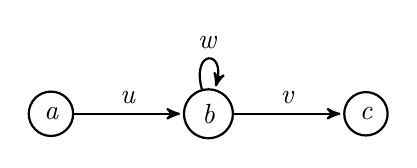
\begin{tikzpicture}[->,>=stealth',shorten >=1pt,auto,node distance=2cm,
                thick,main node/.style={circle,draw,font=\itshape}]
  \node[main node] (a) {\textit{a}};
  \node[main node] (b) [right of=a] {\textit{b}};
  \node[main node] (c) [right of=b] {\textit{c}};

  \path
    (b) edge [loop above] node {\textit{w}} (b)
    (a) edge [above] node {\textit{u}} (b)
    (b) edge [above] node {\textit{v}} (c);      
\end{tikzpicture}
\end{figure}


\noindent
The path capacity from $a$ to $b$ is $u$, from $b$ to $c$ is $v$, and there is a loop at $b$ with capacity $w$. The set of all possible path capacities from $a$ to $c$ is $S = \{ u \otimes v, u \otimes w \otimes v, u \otimes w \otimes w \otimes v, \dots \}$. Our claim is that summing all the elements of $S$,  namely $u \otimes v \oplus u \otimes w \otimes v \oplus u \otimes w \otimes w \otimes v \oplus \dots$, simplifies to $u \otimes v$. In other words, in the presence of boundedness traversing the loop repeatedly does not add any value. Below we show two-elements set $\{ u \otimes v, u \otimes w \otimes v\}$ calculation but we establish it for a general 
setting in the Coq theorem prover.
\begin{align*}
    u \otimes v \oplus u \otimes w \otimes v  
    &= u \otimes (\overline{1} \otimes v \oplus \overline{1} \otimes w \otimes v)\\
    &= u \otimes (v \oplus  w \otimes v)\\
    &=  u \otimes (\overline{1} \oplus  w \otimes \overline{1}) \otimes v \\
    &= u \otimes (\overline{1} \oplus w) \otimes v \\
    &= u \otimes v
\end{align*}


\begin{remark}
    A bounded semiring is also idempotent because boundedness implies $\overline{1} \oplus \overline{1} = \overline{1}$ and multiplying both sides of this equality by $a$ yields $a \oplus a = a$.
\end{remark}


\begin{definition}\label{def:expo}
Let  \( (\mathbb{R}, \oplus, \otimes, \overline{0}, \overline{1}) \) be a semiring. 
We define two operations for $a \in R$ and $k \in \mathbb{N}$: exponentiation ($a^k$) and 
summation-over-$k$-terms ($a^{\langle k \rangle}$), along with their Coq encodings as:
\end{definition}

\begin{minipage}{0.45\linewidth} 
  $a^{k} = 
  \begin{cases}
    \overline{1} & k = 0 \\
    a \otimes a^{k-1} & 1 \leq k  
  \end{cases}$

\begin{lstlisting}[language=Coq]
Fixpoint exp_r (a : R) 
(k : nat) : R := match k with 
| O => 1
| S k' => a * exp_r a k'
end.
\end{lstlisting}
\end{minipage}
  \hfill
\begin{minipage}{0.45\linewidth}{\vspace{3mm}}

$a^{\langle k \rangle} = \overline{1} \oplus a \oplus a^2 \oplus ... \oplus a^k$ 

\begin{lstlisting}[language=Coq]
Fixpoint partial_sum_r (a : R) 
 (k: nat) : R := match k with
 | O => 1
 | S k' => (partial_sum_r a k')  
  + exp_r a k
 end.
\end{lstlisting}
\end{minipage}
\vspace{2mm}




\begin{definition}
 A semiring \( (\mathbb{R}, \oplus, \otimes, \overline{0}, \overline{1}) \) is \textit{k-closed} \cite{10.5555/639508.639512} if there exists a natural number $k$ such that 
 for every $a \in R$: $a^{\langle k + 1 \rangle} = a^{\langle k \rangle}$

\end{definition}

When $k$ = 0, the previous expression simplifies to $\overline{1} + a = \overline{1}$, i.e., the notion of $0$-closed coincides with 
boundedness. In this formalisation, we have assumed  $0$-closed semiring for fixed-point proofs. 

\begin{theorem}\label{bnd}
    Let  \( (\mathbb{R}, \oplus, \otimes, \overline{0}, \overline{1}) \)  be a \textit{k-closed} semiring then we have:  $a^{\langle k + q \rangle} = a^{\langle k \rangle}$ for ever $a \in R$ and for every $q \in \mathbb{N}$. 
    
\end{theorem}
We encode Theorem \ref{bnd} in Coq as \textcolor{blue}{$astar\_exists\_gen\_q\_stable$}. The proof is by induction on $q$ 
and using the fact that it is a $k$-closed semiring. 
\begin{lstlisting}[language=Coq]
Lemma astar_exists_gen_q_stable (k : nat) : (forall w : R, 
 partial_sum_r w k = partial_sum_r w (S k)) -> forall (q : nat) (a : R), 
 partial_sum_r a (q + k) = partial_sum_r a k.
Proof. induction q. (* other proof terms omitted *) Qed.
\end{lstlisting}

\begin{definition}\label{def:inf_sum}
    Let  \( (\mathbb{R}, \oplus, \otimes, \overline{0}, \overline{1}) \)  be a semiring. We define the infinite sum $a^{*}$  of a semiring element  $a \in R$: $a^{*} = \lim_{k\to\infty} a^{\langle k \rangle}$
    
\end{definition}



This is the \textit{closure} of $a$. In general, the infinite sum $a^{*}$ may not always exist. However, in a $k$-closed semiring or 
in a bounded semiring ($0$-closed), this sum is guaranteed to exist. For $k$-closed semirings the infinite sum is $a^{\langle k \rangle}$
(Theorem \ref{bnd} where $a^{*}$ is represented as $a^{\langle q + k \rangle}$ for an arbirary natural number $q$), and 
for bounded semiring the infinite sum is $\overline{1}$. 
Consider the semiring \( (\{false, true\}, \lor, \land, false, true)\), and  in this semiring, 
 $a^{*}$ is equal to $true$, used in graph reachability and the reflexive and transitive closure of binary relations \cite{abdali1985transitive}. We observe that it is a bounded semiring, i.e., 
$true \lor a = true$ ($\overline{1} \oplus a =\overline{1}$ for all $a \in \{false, true\}$).



\subsection{Matrix Semiring}\label{sec:matrix}
We extend the definition of a semiring to a matrix semiring. For a given semiring $(R, \oplus, \otimes, \overline{0}, \overline{1})$ and a natural number $n$, we consider the set of matrices $M_{n}(R)$ of size $n \times n$ with elements in $R$. We define matrix addition, matrix multiplication, and matrix exponentiation (Figure \ref{fig:definitions}), along with their respective Coq encoding (Figure \ref{fig:coq_definitions}).
We define the zero matrix $J$ as a matrix 
with all the entries are $\overline{0}$, and the one matrix (identity matrix) 
$I$ as a matrix with all entries along the diagonal are $\overline{1}$ 
and the rest are $\overline{0}$. The underlying carrier semiring elements and 
their operators induce a 
matrix semiring, i.e., $(M_{n}(R), \oplus_{m}, \otimes_{m}, J, I)$ is a semiring.
We encode the set of matrices $M_{n}(R)$ in Coq as a function type from a finite type to a finite type to \(R\), 
where the finite type is a enumerated list  $finN$, i.e., $finN = \{0, 1, \dots, n-1\}$.
\vspace{-2mm}
\begin{center}
\begin{minipage}{0.7\linewidth}
   \[  (A \oplus_{m} B)_{ij} = A_{ij} \oplus B_{ij} \hspace{2cm} (A \otimes_{m} B)_{ij} = \sum_{k=1}^{n} A_{ik} \otimes B_{kj} \] 
\end{minipage}


\begin{minipage}[t]{0.5\linewidth}
\[(A^k){ij} = \oplus_{r=1}^{n} A_{ir} \otimes (A^{k-1})_{rj}\]
\end{minipage}
\end{center}


\captionof{figure}{Matrix Addition, Matrix Multiplication, and Matrix Exponentiation}
\label{fig:definitions} 



\begin{center}
\begin{minipage}{0.4\linewidth}
\begin{lstlisting}[language=Coq]
Definition matrix_add 
 (A B : Matrix) : Matrix := 
 fun c d => (A c d + B c d).
\end{lstlisting}
\end{minipage}
\hspace{.5cm}
\begin{minipage}{0.4\linewidth}
   \begin{lstlisting}[language=Coq]
Definition matrix_mul 
 (A B : Matrix) : Matrix :=  
 matrix_mul_gen A B finN.
\end{lstlisting}
\end{minipage}
\medskip

\begin{minipage}{0.7\linewidth}{\vspace{2mm}}
\begin{lstlisting}[language=Coq]
Fixpoint matrix_exp_unary (A : Matrix) 
 (k : nat): Matrix := match n with 
 | 0%nat => I 
 | S k' => matrix_mul A (matrix_exp_unary A k')
 end.
\end{lstlisting}
   
\end{minipage}
\end{center}

 \captionof{figure}{Coq Encoding of Matrix Addition, Multiplication, and  Exponentiation}
\label{fig:coq_definitions}
\vspace{2mm}

We use the \textcolor{blue}{$matrix\_exp\_unary$} function for easiness of proofs, but it is 
inefficient for computation ($O(n^3 \times k)$), assuming the matrix $m$ is 
of size $n \times n$. Therefore, we have 
written another function \textcolor{blue}{$matrix\_exp\_binary$}, 
based on the repeated squaring algorithm and proven equivalent to \textcolor{blue}{$matrix\_exp\_unary$}, 
for efficient computation $O(n^3 \times \log{}k)$. 
We would like to emphasise that existing state-of-the-art matrix multiplication algorithms, such as the Strassen algorithm \cite{strassen1969gaussian} and the Coppersmith-Winograd algorithm \cite{COPPERSMITH1990251}, do not apply to semirings in general because semirings lack a subtraction operator.
 There are some algorithms \cite{vassilevska2009all,10.1145/3186893}
with subcubic time complexity for specialised semirings but they are mostly for theoretical interests. 


\begin{theorem}\label{one} 
    \((M_{n}(R),  \oplus_{m}, \otimes_{m}, J, I)\) is a semiring when 
    the underlying carrier set 
    \((R, \oplus, \otimes, \overline{0}, \overline{1})\) is a 
    semiring.
\end{theorem}



\begin{theorem}\label{two}
    \((M_{n}(R),  \oplus_{m}, \otimes_{m}, J, I)\) is an idempotent 
    semiring when the underlying carrier set \((R, \oplus, \otimes, \overline{0}, \overline{1})\) is an idempotent semiring.
\end{theorem}

The proofs of Theorem \ref{one} and Theorem \ref{two} follow from the properties the  underlying carrier set $R$. 
However, when the underlying carrier set \(R\) is a bounded semiring, the induced matrix semiring \((M_{n}(R), \oplus_{m}, \otimes_{m}, J, I)\) is \((n-1)\)-closed. This means that for a given matrix \(A \in M_{n}(R)\), it holds that \(A^{\langle n - 1 \rangle} = A^{\langle k + n - 1 \rangle}\) for an arbitrary natural number \(k\) (Theorem \ref{thm:thm4}). Furthermore, with the more general assumption of idempotence, we can efficiently compute \(A^{\langle n - 1 \rangle}\) using matrix exponentiation (Theorem \ref{thm:thm3}).







\begin{definition}
   Let   \((M_{n}(R),  \oplus_{m}, \otimes_{m}, J, I)\) is a semiring.
   For every $A \in M_{n}(R)$ and for every $k \in \mathbb{N}$, we define the formal power series $A^{\langle k \rangle}$, 
   along with its Coq encoding: $A^{\langle k \rangle} = I \oplus_{m} A \oplus_{m} A^2 \oplus_{m} \ldots \oplus_{m} A^k$.
\end{definition}
\begin{lstlisting}[language=Coq]
Fixpoint partial_sum_mat (A : Matrix) (k : nat) : Matrix := 
 match k with
 | O => I 
 | S k' => (partial_sum_mat A k') +M (matrix_exp_unary A k)
end.
\end{lstlisting}
%\vspace{-2mm}
  %\caption{Formal (Matrix) Power Series}
%\label{eq:matrix_sum_upto_k}

%\vspace{2mm}


We can compute the formal power series $A^{\langle k \rangle}$  efficiently in 
$O(n^3 \times (\log{}k)^2)$ using Equation (\ref{eq:myequation}), compared to naive $O(n^3 \times k^2)$ of \textcolor{blue}{$partial\_sum\_mat$}, assuming that $A$ is a  $n \times n$ matrix.
Our focus, however, lies in computing $A^{*}$, the 
generalised Kleene star \cite{Droste2009}. 

\begin{equation}
A^{\langle k \rangle} = 
\begin{cases}
    I & \text{if } k = 0 \\
    A^{\langle k / 2 \rangle} \otimes_{m} (I \oplus_{m} A^{ (k / 2) + 1}) & \text{if } k \text{ is odd} \\
    A^{\langle (k / 2) - 1\rangle} \otimes_{m} (I \oplus_{m} A^{k / 2}) \oplus_{m} A^k & \text{if } k \text{ is even} 
\end{cases}
\label{eq:myequation}
\end{equation}
%\vspace{1mm}
\begin{definition}\label{eq:matrix_sum_infinite}
Let   \((M_{n}(R),  \oplus_{m}, \otimes_{m}, J, I)\) is a semiring.
   For ever $A \in M_{n}(R)$, we define  the 
infinite sum $A^{*}$ as: 
$\quad A^{*} = \lim_{k\to\infty} A^{\langle k \rangle}$.
\end{definition}


This is the closure of $A$. We have not encoded $A^{*}$ in Coq because we do not want to compute it. In many cases, computing $A^{*}$ is a diverging process; for example, with regular languages endowed with the concatenation and union operators, it never reaches a fixed point. We are only interested in cases where $A^{*}$ is well-defined and does reach a fixed point. Therefore, we express $A^{*}$ as 
$A^{\langle k + n - 1 \rangle}$ in proofs, where  $k$  is an arbitrary natural number and $n$ is the dimension of $A$. Ideally, we could have encoded $A^{*}$ as a coinductive definition and demonstrated that it reaches a fixed point using a mix of inductive and coinductive reasoning \cite{Nakata_2010}. However, this would have complicated our reasoning without significant benefit.



\section{Kleene Star and Fixed Points}
\label{sec:kleene}
The expression $A^{*}$ represents the Schulze method with appropriate instantiated operators. More precisely, the underlying semiring is 
$(N^{\infty}, max, min, 0, \infty)$ where $N^{\infty} = N \cup \{\infty\}$, $A$ is the margin matrix and $A^{*}$  is the generalised margin matrix of the Schulze method.  Fortunately, the Schulze method can be generalised to a bounded semiring 
-- $max(a, \infty) = \infty \text{ for every } a \in N^{\infty}$ -- which insures the existence of 
a fixed point, i.e., $A^{*} = A^{\langle n - 1 \rangle}$. 


\subsection{Primary Results} 
Theorem \ref{thm:thm4} states that in a bounded semiring, 
the limit of infinite sum $A^{*}$ is well-defined  and it is equal to $A^{\langle n - 1 \rangle}$.
Moreover, we can compute  $A^{\langle n - 1 \rangle}$ efficiently using the 
matrix exponentiation method (Theorem \ref{thm:thm3}) by computing 
$(A \oplus I)^{(n - 1)}$ (Theorem \ref{thm:thm5}).



\begin{theorem}\label{thm:thm4}
Let \( (\mathbb{R}, \oplus, \otimes, \overline{0}, \overline{1}) \) be a bounded semiring. Then the matrix semiring \( (M_{n}(\mathbb{R}), \oplus_{m}, \otimes_{m}, J, I) \) is \((n-1)\)-closed, meaning that for every \( A \in M_{n}(\mathbb{R}) \) and \( k \in \mathbb{N} \), it holds that \( A^{\langle k + n - 1 \rangle} = A^{\langle n - 1 \rangle} \).


\end{theorem}

We encode Theorem \ref{thm:thm4} in Coq as \textcolor{blue}{$zero\_stable\_partial$}, assuming a bounded semiring which is represented by \textcolor{blue}{$zero\_stable$}. Essentially, we reduce this fixed-point proof to another fixed-point proof, \textcolor{blue}{$sum\_all\_flat\_paths\_fixpoint$}, as it provides additional information and structure. A detailed explanation of \textcolor{blue}{$sum\_all\_flat\_paths\_fixpoint$} is given in Section \ref{sec:graph}.





\begin{lstlisting}[language=Coq]
Theorem zero_stable_partial n (zero_stable : forall a : R, 1 + a = 1) : 
 forall (k : nat) (A : Matrix Node R) (c d : Node),   
 partial_sum_mat A (k + n - 1) c d = partial_sum_mat  A (n - 1) c d.
Proof. eapply sum_all_flat_paths_fixpoint.(* other terms omitted *) Qed.
\end{lstlisting}
%\captionof{figure}{Formal Power Series Fixed Point}
%\label{fig:formalfixpoint} 

\begin{theorem}\label{thm:thm3}
    Let \((M_{n}(R),  \oplus_{m}, \otimes_{m}, J, I)\) be an idempotent 
    semiring and $A \in M_{n}(R)$, 
    then we have  $A^{\langle k \rangle} = (A \oplus I)^k$.
\end{theorem}

We encode Theorem \ref{thm:thm3} in Coq as \textcolor{blue}{$matrix\_pow\_idempotence$}, which connects matrix exponentiation to the formal power series. The proof for this theorem is by induction on \(k\). We can compute \(A^{\langle k \rangle}\) in \(O(n^3 \times \log{k})\) using matrix exponentiation --compared to \(O(n^3 \times (\log{k})^2)\)-- under the assumption of idempotence. 
This efficiency stems from the connection between idempotent semirings and dynamic programming, where idempotency ensures that only optimal substructures contribute to the final solution \cite{10.5555/639508.639512}.
Mohri \cite{10.5555/639508.639512} explains the connection between the optimal substructure property of dynamic programming algorithms and the monotonicity property of semirings. Idempotency introduces a partial order, which in turn makes a semiring monotonic.



\begin{lstlisting}[language=Coq]
Theorem matrix_pow_idempotence  (plus_idempotence : forall a : R, 
  a + a = a) : forall (k : nat) (A : Matrix Node R) (c d : Node),
  partial_sum_mat A k c d = matrix_exp_unary (A +M I) k c d.
Proof. induction k. (* other terms omitted *) Qed.
\end{lstlisting}

\begin{theorem}\label{thm:thm5}
    Let \((M_{n}(R),  \oplus_{m}, \otimes_{m}, J, I)\) be a \((n-1)\)-closed
    semiring and $A \in M_{n}(R)$, 
    then we have  $(A \oplus I)^{k + n - 1} = (A \oplus I)^{n - 1} $ {for every} $k \in N$. 
\end{theorem}    

It is a consequence of Theorems \ref{thm:thm4} and \ref{thm:thm3}.
We encode Theorem \ref{thm:thm5} in Coq as \textcolor{blue}{$matrix\_fixpoint$}. Note 
that boundeness implies idempotence. 

\begin{lstlisting}[language=Coq]
Theorem matrix_fixpoint n (zero_stable : forall a : R, 1 + a = 1) : 
 forall k A c d, matrix_exp_unary (A +M I)  (n - 1) c d =  
 matrix_exp_unary (A +M I) (k + n - 1) c d.
Proof. 
    (* some proofs terms omitted *)
    rewrite (matrix_pow_idempotence  k A c d).
    rewrite (matrix_pow_idempotence  (k + n - 1) A c d).
    eapply zero_stable_partial.
Qed.
\end{lstlisting}


\subsection{Graph Theory}\label{sec:graph} 
In this section, we present the proof of \textcolor{blue}{$sum\_all\_flat\_paths\_fixpoint$}, 
expressed as Theorem \ref{thm:thm8}. 
We interpret a square matrix $A \in M_{n}(R)$ as a graph \( G = (V, E) \), where the set of vertices is \( V \) = \{1, \ldots, $n$\} and the set of edges is \( E = \{x \in V \times V\}\). Each entry $A_{ij}$ corresponds to the weight of the edge from vertex $i$ to vertex $j$. The cost of a path \(\pi = (v_0, \ldots, v_k)\) in $G$ is defined as $A(v_0, v_1)\otimes A(v_1, v_2) \otimes \ldots \otimes A(v_{k-1}, v_{k})$. More generally, we express this as $\textcolor{blue}{measure\_of\_path}(\pi) = \bigotimes_{e \in \pi} \text{ }A(e)$, where the product is taken over all edges $e$ in the path $\pi$.
Similarly, the cost of a set of paths $P$ is defined as the sum of the costs of all individual paths in $P$ and  expressed as: $ \textcolor{blue}{sum\_all\_rvalues} (P) = 
  \bigoplus_{\pi \in P} \text{ } \textcolor{blue}{measure\_of\_path} (\pi)$. The Coq encodings of these definitions are shown below, where the cost of an empty path (\(\epsilon\)) is represented by \(\overline{1}\), and the cost of an empty set (\(\{\}\)) is denoted by \(\overline{0}\).

\vspace{2mm}
\begin{minipage}[t]{0.48\linewidth}
\begin{lstlisting}[language=Coq]
Definition measure_of_path 
 (p : Path) : R := fold_right 
 (fun '(_, _, b) a => b * a) 1 
 p
\end{lstlisting}
\end{minipage}
\hspace{3mm}
\begin{minipage}[t]{0.45\linewidth}{\vspace{-2mm}}
\begin{lstlisting}[language=Coq]
Definition sum_all_rvalues 
 (pl : list Path) := fold_right 
 (fun b a => b + a) 0 
  (map (fun '(_, _, p) => 
   measure_of_path p) pl).
    \end{lstlisting} 
    %Rew1:Syntax error in fun'(_, _, l) =>
  \end{minipage}
 \vspace{4mm} 

We interpret $A^k$ and $A^{\langle k \rangle}$ in terms of 
a set of paths.
Intuitively $A^{1}$ represents the cost 
of the set of the unit length paths in $G$, $A^{2}$ represents 
the cost of the set of two length paths in $G$, so on and so forth. 
More generally, the value $A^{k}_{ij}$ --row $i$ and column $j$ in matrix $A^{k}$-- 
represents the cost of the set of paths from $i$ to $j$ with exactly $k$ arcs,
and the value $A^{\langle k \rangle}_{ij}$ represents the cost of the set of paths 
from $i$ to $j$ with \textit{at most} $k$ arcs. 
We make this observation more formal and define a recursive function $P^{k}(i, j)$
that computes the set of paths from $i$ to $j$ with exactly $k$ arcs.
This formalisation is illustrated on the left side and its corresponding Coq encoding is presented on 
the right side of Figure \ref{fig:definitionofpaths}. 
The Coq encoding takes two 
extra argument the adjacency matrix $A$ and its size $n$, 
enumerated in a list $finN$, i.e., $finN = \{0, 1, \dots, n-1\}$. 
This is because we encode a path $(c, c_1, c_2 \dots )$ in Coq as a list 
$[(c, c_1, A(c, c_1)); (c_1, c_2, A(c_1, c_2)); \dots ]$.
This representation allows us to easily calculate the path weight by traversing the path. 


\begin{center}
\begin{minipage}[t]{0.45\textwidth}

 \[
P^{0}(i, j) = 
\begin{cases}
    {\{\epsilon\}} & i = j \\
    \{\} & i \neq j 
\end{cases}
\]
\[
P^{k+1}(i, j) = \cup_{q = 1}^{n} (i, q) \odot P^{k}(q, j)
\] where $\odot$ is an append operation which takes a pair of nodes and 
a set of paths and appends the pair of nodes to 
every path in the set of paths. 
\end{minipage}
\hfill
\begin{minipage}[t]{0.48\textwidth}{\vspace{-2mm}}
 \begin{lstlisting}[language=Coq]
Fixpoint all_paths_klength 
 (finN : list Node) (A : Matrix) k 
 (c d : Node) : list Path :=
 match k with
 | O => if c =n= d then 
  [[(c, d, 1)]] else []
 | S k' => let lf := flat_map 
   (fun x => all_paths_klength 
    finN A k' x d) finN in 
   append_node_in_paths A c lf
 end.
    \end{lstlisting}
\end{minipage}

\captionof{figure}{Definition of Path Set (left) and its Coq Encoding (right)}
\label{fig:definitionofpaths}
\end{center}

Furthermore, we define $P^{\langle k \rangle}(i, j)$, the set of path sets,
be the set of paths from $i$ to $j$ with  at most $k$ arcs as 
$ P^{\langle k \rangle}(i, j) = \cup_{t = 0}^{k}\text{ } P^{t}(i, j)$ with the coq encoding 
\textcolor{blue}{$enum\_all\_paths\_flat$}.
\vspace{2mm}
%\begin{center}
\begin{lstlisting}[language=Coq]
(* Get all the paths in one big list *)
Fixpoint enum_all_paths_flat (finN : list Node) (A : Matrix Node R) 
(n : nat) (c d : Node) : list Path := match n with
 | O => all_paths_klength finN A O c d
 | S n' => all_paths_klength finN A n c d ++ 
   enum_all_paths_flat finN A n' c d
 end.
\end{lstlisting}
%\captionof{figure}{The Set of Path Sets with at most k arcs}
\label{fig:defpath}
%\end{center}


More concretely, \textcolor{blue}{$all\_paths\_klength$}  $finN$ $A$ $k$  $i$  $j$ constructs the set $P^{k}(i, j)$
and \textcolor{blue}{$enum\_all\_paths\_flat$} $finN$ $A$ $k$  $i$  $j$ constructs the set $P^{\langle k \rangle}(i, j)$.
We formally establish in Coq that $A^{k}(i, j) = \bigoplus_{p \in P^{k}(i, j)} \, \textcolor{blue}{measure\_of\_path}(p)$, expressed 
 as  \textcolor{blue}{$matrix\_path\_equation$}, and  
 $A^{\langle k \rangle}(i, j) = \bigoplus_{p \in P^{\langle k \rangle}(i, j)} \text{ } \textcolor{blue}{measure\_of\_path}(p)$, expressed as \textcolor{blue}{$matrix\_ppath\_equation$}. 
 While the proof follows a straightforward induction on $k$, these equations offer a more detailed and structured way to reason about matrix exponentiation and formal power series in terms of paths. This interpretation precisely allows us 
to connect the fixed-point proof expressed in terms of paths, Theorem \ref{thm:thm8}, 
 to the fixed-point proof expressed in terms of the formal power series, Theorem \ref{thm:thm4}.
 
 
 \begin{lstlisting}[language=Coq]
Lemma matrix_path_equation (finN : list Node) : forall k A i j,
 matrix_exp_unary A k i j = 
 sum_all_rvalue (all_paths_klenght finN A k i j)).
Proof. (* proof terms omitted *) Qed.

Lemma matrix_ppath_equation (finN : list Node) : forall k A c d,
 partial_sum_mat A k i j = 
 sum_all_rvalue (enum_all_paths_flat finN A k i j)). 
Proof.  (* proof terms omitted *) Qed. 
\end{lstlisting}

 
\begin{theorem}\label{thm:thm8}
Let \((R, \oplus, \otimes, \overline{0}, \overline{1})\) be a bounded 
semiring. In a graph with $n$ nodes where the edge costs are drawn from $R$, the following holds 
for all $k \in N$.
\end{theorem}
\[  
\bigoplus_{p \in P^{\langle n - 1 \rangle}(i, j)}\;\textcolor{blue}{measure\_of\_path}(p)  =  
\bigoplus_{p \in P^{\langle k + n - 1 \rangle}(i, j)}\;\textcolor{blue}{measure\_of\_path}(p)
\]   





Theorem \ref{thm:thm8} formalises the idea that iterating through loops becomes redundant in presence of boundedness. 
The proof proceeds by induction on $k$, with a trivial base case, but the inductive case requires careful exposition. 
In the inductive step, the hypothesis is 
$ \bigoplus_{p \in P^{\langle n - 1 \rangle}(i, j)} \, \textcolor{blue}{measure\_of\_path}(p) = 
\bigoplus_{p \in P^{\langle k + n - 1 \rangle}(i, j)} \, \textcolor{blue}{measure\_of\_path}(p)$ and the goal is to establish the fact that $ \bigoplus_{p \in P^{\langle n - 1 \rangle}(i, j)} \, \textcolor{blue}{measure\_of\_path}(p) =  
   \bigoplus_{p \in P^{\langle k + n - 1 + 1 \rangle}(i, j)} \, \textcolor{blue}{measure\_of\_path}(p)$. 
We simplify the expression $\bigoplus_{p \in P^{\langle k + n - 1 + 1 \rangle}(i, j)} \, \textcolor{blue}{measure\_of\_path}(p)$ as 
$\bigoplus_{p \in P^{\langle k + n - 1 \rangle}(i, j)} \ \textcolor{blue}{measure\_of\_path}(p) \oplus \bigoplus_{p \in P^{k + n - 1 + 1}(i, j)} \ \textcolor{blue}{measure\_of\_path}(p)$ by following 
the definition of  $P^{\langle k \rangle}(i, j)$  and using the fact the $\textcolor{blue}{measure\_of\_path}(\{p_{1}, p_{2} \}) = 
\textcolor{blue}{measure\_of\_path}(p_{1}) \oplus \textcolor{blue}{measure\_of\_path} (p_{2})$. However, if the path  $p_{2}$ is identical to  $p_{1}$ but contains an additional loop, i.e.,
$\textcolor{blue}{measure\_of\_path}(p_{1}) = a \otimes b$ and $\textcolor{blue}{measure\_of\_path}(p_{2}) = a \otimes c \otimes b$, 
then $\textcolor{blue}{measure\_of\_path}(p_{1}) \oplus \textcolor{blue}{measure\_of\_path}(p_{2})$ simplifies to $\textcolor{blue}{measure\_of\_path}(p_{1})$ due to boundedness. 
Given that there are $n$ nodes, we establish that every path $p \in P^{k + n - 1 + 1}(i, j)$ contains a loop, so 
these loops can be reduced, allowing the paths to be subsumed into the set $P^{\langle k + n - 1 \rangle}(i, j)$.
More precisely, $\bigoplus_{p \in P^{\langle k + n - 1 \rangle}(i, j)} \ \textcolor{blue}{measure\_of\_path}(p) \oplus \bigoplus_{p \in P^{ k + n - 1 + 1}(i, j)} \ \textcolor{blue}{measure\_of\_path}(p)$
simplifies to $\bigoplus_{p \in P^{\langle k + n - 1 \rangle}(i, j)} \ \textcolor{blue}{measure\_of\_path}(p)$ and this is precisely the induction hypothesis. 
We encode Theorem \ref{thm:thm8} in Coq as below and in the inductive case, 
it relies on \textcolor{blue}{$sum\_all\_flat\_paths\_idempotence$} which mimics the 
$\bigoplus_{p \in P^{\langle k + n - 1 \rangle}(i, j)} \ \textcolor{blue}{measure\_of\_path}(p) \oplus \bigoplus_{p \in P^{k + n - 1 + 1}(i, j)} \ \textcolor{blue}{measure\_of\_path}(p)$
simplifies to $\bigoplus_{p \in P^{\langle k + n - 1 \rangle}(i, j)} \ \textcolor{blue}{measure\_of\_path}(p)$ (\emph{Orel a b} is defined as $a + b = a$).
\vspace{2mm}
\begin{lstlisting}[language=Coq]
Lemma sum_all_flat_paths_fixpoint(zero_stable : forall a : R, 1 + a = 1):  
 forall (k : nat) (A : Matrix Node R) (c d : Node), 
 sum_all_rvalues (enum_all_paths_flat finN A (length finN - 1) c d) =
 sum_all_rvalues (enum_all_paths_flat finN A (k + length finN - 1) c d).
Proof. 
 induction k as [| k IHk]
 + reflexivity.
 + (* inductive case *)
   (* some proof terms omitted *) 
   rewrite sum_all_flat_paths_idempotence. 
   exact IHk.
   ....
Qed.

Lemma sum_all_flat_paths_idempotence : forall (la lb : list Path), 
(forall (xs : Path), In_path_membership xs la = true -> exists ys, 
 In ys lb = true /\  Orel (measure_of_path ys) (measure_of_path xs)) ->
 Orel (sum_all_rvalues lb) (sum_all_rvalues la).           
Proof.  (* proof terms omitted *) Qed.
\end{lstlisting}
\section{Application: Schulze Voting Method}
\label{sec:schulze-experiment}\label{sec:schulze-experiment}
%\vspace{-1.5cm}
We demonstrate the usability of our formalisation by verifying the Schulze elections as explained on its 
Wikipedia page \cite{schulze-wikipedia} and in the original paper \cite{schulze2011new}, 
but we show here only the Coq encoding of the Wikipedia example. This choice is intentional because the Wikipedia page has been scrutinised by many experts, including Markus Schulze himself, making it a reliable example. We define the candidates
as an inductive datatype $Node$.  For pairwise preferences, we define an inductive datatype \(R\) with two constructors: \(Left\) and \(Infinity\). \(Left\) takes a natural number representing the pairwise preferences between two candidates, 
while \(Infinity\) is used when no preference exists between the candidates (a candidate is not preferred over itself so 
preference over itself is \(Infinity\)).
Next, we define $zero$, $one$, $plus$, and $mul$ and use them to construct an election \textcolor{blue}{$wikipedia$} that calls $\textcolor{blue}{matrix\_exp\_binary}$ (Figure \ref{fig:coq}). Since 
we have 5 candidates, the fixed point will reach in 4 iterations; hence the number 4 in $\textcolor{blue}{matrix\_exp\_binary}$. We discharge --not 
shown here-- all the axioms of semiring, including boundedness. In order to get an executable machine code, we extract the \textcolor{blue}{$wikipedia$} function into an OCaml code using the Coq's extraction facility and call it from 
the main OCaml file with the (margin) matrix that represents the pairwise preferences of voters (Figure \ref{fig:ocaml}). 

\begin{minipage}{0.45\linewidth}{\vspace{5mm}}
\begin{lstlisting}[language=Coq]
Inductive Node := 
 A | B | C | D | E. 

Inductive R :=
| Left : nat -> R
| Infinity : R.
  
Definition zero : R := 
 Left 0.

Definition one : R := 
 Infinity.

Definition plus (u v : R) :=
match u, v with 
| Left x, Left y => 
  Left (Nat.max x y) 
| _, _ => Infinity
end.
\end{lstlisting}
\end{minipage}
\hspace{2mm}
\begin{minipage}{0.5\linewidth}{\vspace{3mm}}
\begin{lstlisting}[language=Coq]
Definition mul (u v : R) : R :=
match u, v with 
| Left x, Left y => 
  Left (Nat.min x y)
| Left x, Infinity => Left x 
| Infinity, Left y => Left y 
| _, _ => Infinity 
end.

Definition finN : list Node :=
 [A; B; C; D; E].

Definition wikipedia 
 (m : Matrix Node R) :=
 matrix_exp_binary finN zero 
 one m 4.


 
\end{lstlisting}
\end{minipage}
\captionof{figure}{Coq Encoding of the Schulze Election from Wikipedia}
\label{fig:coq}
\begin{center}
\begin{minipage}[t]{0.7\linewidth}{\vspace{- 3.9mm}}
\begin{lstlisting}[language=Caml]
let matrix : coq_R array array = 
[|
 [| one; Left 20; Left 26; Left 30; Left 22|];
 [| Left 25; one; Left 16; Left 33; Left 18|];
 [| Left 19; Left 29; one; Left 17; Left 24|];
 [| Left 15; Left 12; Left 28; one; Left 14|];
 [| Left 23; Left 27; Left 21; Left 31; one|]
|]

let _ = 
  let comp = wikipedia matrix in 
  let ret = .... in 
  print_endline (string_list ret)
\end{lstlisting}
\end{minipage}
\end{center}
%\vspace{-1cm}
\captionof{figure}{Toplevel OCaml code with Matrix Configuration}
\label{fig:ocaml} 


\section{Further Applications}
\label{sec:applications}
While our primary aim is to unify the Schulze method within the semiring framework, the abstract nature of our formalisation also encompasses a wide range of other examples, ranging from traditional computer science to mathematics.



\subsection{Optimisation (Widest-Shortest Path)}
Consider a graph where each edge, representing a link, has a weight in the form of a pair, with the first element representing the delay and the second element representing the bandwidth of the link. Our objective is to compute the shortest paths between two given nodes, minimising delay. However, if multiple such paths exist, we prioritise selecting the one with the greatest bandwidth \cite{baras2022path}. We can see this problem as an optimisation problem with two data points, and we encode this problem in our framework 
as the semiring $(R, \oplus, \otimes, \overline{0}, \overline{1})$ where 
$R = N^{\infty} * N^{\infty} \text{ where }N^{\infty} = N \cup\{\infty\}$, $\oplus$ is defined as  Equation \ref{eq:semiring-addition}, 
$\otimes$ is defined as Equation \ref{eq:semiring-multiplication}, 
$\overline{0}$ is defined as (0, $\infty$), and 
$\overline{1}$ is defined as ($\infty$, 0).



\begin{equation}\label{eq:semiring-addition}
  (d_1, b_1) \oplus (d_2, b_2) = 
  \begin{cases}
    (d_1, b_1) & \text{if } d_1 < d_2 \text{ or } (d_1 = d_2 \text{ and } b_2 < b_1) \\
    (d_2, b_2) & \text{otherwise}   
  \end{cases}
\end{equation}


\begin{equation}\label{eq:semiring-multiplication}
  (d_1, b_1) \otimes (d_2, b_2) = (d_1 + d_2, \min(b_1, b_2)).
\end{equation}


We have encoded this algorithm in our framework (see Appendix \ref{appendix}). In addition, 
we can generalise this over an objective with $n$ entries with
appropriate definitions to solve a multi-objective problem \cite{manger2020algebraic}. 



\subsection{Social Network (Geodetic Semiring)}
Assume a graph that models a community \cite{baras2022path,batagelj1994semirings}. In this graph, each edge weight is a pair where 
the first element of the pair indicates the length of the shortest paths between two nodes, while the second element denotes the number of such paths. Our aim is to compute the closeness between community members.
This problem can be encoded within our framework using the semiring  $(R, \oplus, \otimes, \overline{0}, \overline{1})$, 
where $R = N^{\infty} \times N^{\infty}$, $\oplus$ is defined as Equation \ref{ceq_plus}, 
$\otimes$ is defined as Equation \ref{ceq_mul}, $\overline{0}$ is defined 
$(\infty, 0)$, and $\overline{1}$ is defined $(0, 1)$.


\begin{equation}\label{ceq_plus}
    (d_1, n_1) \oplus (d_2, n_2) =
    \begin{cases}
    (d_1, n_1) & \text{if } d_1 < d_2  \\
    (d_2, n_2) & \text{if } d_2 < d_1  \\
    (d_1, n_1 + n_2) & \text{otherwise}   
  \end{cases}
\end{equation}

\begin{equation}\label{ceq_mul}
    (d_1, n_1) \otimes (d_2, n_2) = (d_1 + d_2, n_1*n_2)
\end{equation}


\subsection{Machine Learning (Expectation Semiring)}
Imagine a graph where each edge is represented by a pair $(p, v)$, where $p$ denotes the probability of traversing the edge and $v$ represents the cost of traversing the edge. The total cost accumulates additively along a path \cite{baras2022path,10.3115/1073083.1073085,10.1007/11682462_32}. Additionally, we require that $\Sigma_j p_{ij} = 1$, meaning the sum of the probabilities of all edges originating from node $i$ is equal to 1. Our goal is to compute the expected value of paths from vertex $s$ to vertex $t$. We can encode this problem in our framework 
using the semiring $(R, \oplus, \otimes, \overline{0}, \overline{1})$ where 
$R = \mathcal{R} \times \mathcal{R}$, $\oplus$ is defined as Equation \ref{eq_plus}, 
$\otimes$ is defined as Equation \ref{eq_mul}, $\overline{0}$ is defined 
$(0, 0)$, and $\overline{1}$ is defined $(1, 0)$.


\begin{minipage}{0.45\textwidth}
\begin{equation}\label{eq_plus}
(a, b) \oplus (c, d) = (a + c, b + d)
\end{equation}
\end{minipage}
\hfill
\begin{minipage}{0.45\textwidth}
\begin{equation}\label{eq_mul}
(a, b) \otimes (c, d) = (ac, ad + bc)
\end{equation}
\end{minipage} 

\section{Related Work}
\label{sec:related}
Semirings have found their place in almost every part of computer science, including networking \cite{10.1145/3387514.3405864,10.1145/3332466.3374533,10.1145/3230543.3230561}, optimization \cite{manger2020algebraic}, parsing \cite{10.5555/973226.973230,opedal-et-al-2023,10.5555/1609067.1609126}, social networks \cite{10.1145/2959100.2959148}, social choice \cite{Rossi2011,pini2013resistance}, logic \cite{10.1145/3531130.3533358}, databases \cite{10.1145/1265530.1265535,10.1145/2448496.2448516,10.5555/3319379.3319390,10.14778/3236187.3236200,10.14778/2140436.2140445,10.1145/3477314.3507687}, program analysis \cite{esparza2010newtonian,kincaid2021algebraic,10.1145/3453483.3454079,10.1145/3591280,10.1145/3341644}, runtime verification \cite{jakvsic2018algebraic}, reversible programming \cite{10.1007/978-3-662-49498-1_6}, and machine learning \cite{pmlr-v162-sanmarti-n22a,7888519,10.1145/3583133.3590747,10.1162/COLI_a_00198,roark2011lexicographic}. Given their wide usage, there are a few open-source implementations, e.g., C++ \cite{10.1007/978-3-319-08846-4_1,10.1007/978-3-642-45221-5_48,10.1145/3322125,10.1007/978-3-540-76336-9_3} and Haskell \cite{10.1145/2544174.2500613,erwig2021explainable}. None of these implementations, however, have been proven correct and offer no formal guarantees. There are existing works that formalise Kleene Algebra \cite{10.1007/978-3-642-14052-5_13,MOREIRA2015377} in Coq 
for developing a tactic for deciding the equational theory of Kleene algebras. Kleene algebras are idempotent semirings that include the Kleene star operator.  In contrast, we assume a bounded semiring and prove that the Kleene star (formal power series) always reaches a fixed point. The Schulze method has been formalised by Pattinson et al. \cite{pattinson2017schulze} using the Coq theorem prover. From this formalisation, they extracted Haskell code capable of counting 100,000 ballots with 4 candidates. 
In a subsequent paper, Moses et al. \cite{10.1007/978-3-319-68687-5_5} improved the runtime of this implementation, capable of counting 8 million ballots with 4 candidates.
Both formalisations involve the concrete $maximum$ and $minimum$ function of the Schulze method and 
therefore  require a lot of reasoning about these functions. On the contrary, we do not formalise the 
Schulze method but the formal power series (Kleen star) in semirings and the Schulze method is just an instance of it. 
Our abstraction allows us to reason only in terms of semiring axioms and thereby eliminating all the unnecessary details.
Moreover, our formalisation is amenable to parallelisation by means of matrix multiplication \cite{chang2022revisiting}.
In a nutshell,  our formalisation subsumes the work of Pattinson et al. \cite{pattinson2017schulze} and Moses et al. \cite{10.1007/978-3-319-68687-5_5}. Csar et al.  \cite{10.5555/3304415.3304442} have designed Pregel framework, inspired by Valiant’s Bulk Synchronous Parallel model \cite{10.1145/79173.79181}, to compute the Schulze winner for large number of preferences. 
Again, \cite{10.5555/3304415.3304442} is written in C++ so offers no formal 
guarantees about the correctness of the output. Haines et al. \cite{haines2019verifiable} developed the first homomorphic tallying system for the Schulze method. \cite{haines2019verifiable} assumes the existence of a finite field, a standard cryptographic assumption, meanwhile we work in a very impoverish algebraic structure of semiring. 



\vspace{2mm}
One of the bottlenecks of our work is its complexity $O(n^3 \times log\text{ }n)$, where 
$n$ is the number of candidates, for producing the Schulze winner, while algorithm 
given by Schulze \cite{schulze2011new} has $O(n^3)$ complexity. We could have 
generalised the Schulze method to 
semirings to get the desired complexity of $O(n^3)$, but going 
for matrix representation and incurring an extra $log$ factor was 
a deliberate choice. The Schulze method is not amenable to 
parallelisation for applications that involves large number of 
preferences \cite{10.5555/3304415.3304442}, meanwhile 
matrix multiplication can be parallelised easily by using 
GPU \cite{chang2022revisiting}.
A further limitation of our work is that it assumes the knowledge 
of the Coq theorem prover to use our library,  specifically discharging the 
axioms of semiring after instantiating the $\oplus$ and $\otimes$. 
This, however, could be challenging with the semirings that has been 
obtained by combining multiple semirings 
and therefore we would like to automate this process in the future work.
Better yet, we allow users to instantiate the $\oplus$ and $\otimes$ 
with their operators and the library automatically proves if 
the operators follow the semiring axiom or not. If not, then it produces 
a counter example for the user. This feature specially will be helpful in 
situations where  the semirings 
obtained by combining multiple semirings, e.g., geodetic semiring, 
multi-objective optimisation \cite{manger2020algebraic}, etc.  



\vspace{2mm}
In future work, we aim to formally verify that our formalisation possesses all key social choice properties, such as the Condorcet winner criterion, monotonicity, 
reversal symmetry, pareto, etc.,  
established by Schulze \cite{schulze2011new} using the Coq theorem prover.
There is some effort by Tiwari et al. \cite{Tiwari2021b} to 
establish Condorcet winner and reversal symmetry about their implementation \cite{pattinson2017schulze},
but it is not complete. Moreover, their approach is more complicated 
because they need to deal with details of \emph{maximum} and 
\emph{minimum} function 
over integers, meanwhile our formalisation has abstracted all the details into 
semiring and therefore most of the social choice proofs 
can easily be established in Coq. Another future 
work we would like to extend our matrix multiplication 
to parallelisation using the SyDPaCC \cite{10.1145/3605156.3606450} library 
and use this library for computing the Schulze winner for 
large number of preferences \cite{10.5555/3304415.3304442}. 
Another possible research direction is including more algorithms such 
as generalised graph algorithms on semiring \cite{10.5555/639508.639512,GUTTMANN201837}. 
Furthermore, our matrix representation is defined as a function type, which simplifies proofs but is 
inefficient for execution. To enhance performance, we plan to improve it using a refinement-based approach \cite{10.1007/978-3-642-32347-8_7}. 
Moreover, given that Kleene algebra is an instance of 
idempotent semiring, another possibility is to prove that our implementation 
follows all the axioms of Kleene algebra. 
We can extend our formalisation to algebraic program analysis \cite{esparza2010newtonian,kincaid2021algebraic}, 
assuming $\omega$-continuous semiring. Finally, by adding 
semimodule \cite{Głazek2002,Golan1999,10.5555/1386688} in our formalisation, we can capture more 
applications, e.g., discrete event system \cite{baccelli1992synchronization}, 
data mining \cite{10.1007/978-3-540-70901-5_12}, 
image processing \cite{10.1016/j.ins.2006.09.002}, etc. 




%%
%% Bibliography
%%

%% Please use bibtex, 


\section{Semimodules}
\label{sec:semimodules}

A \emph{left semimodule} over a semiring $(R, \oplus, \otimes, \overline{0}, \overline{1})$
is a commutative monoid $(M, \oplus_M, 0_M)$ equipped with a scalar multiplication
$\odot : R \times M \to M$ satisfying:
\begin{align*}
(a \oplus b) \odot x &= (a \odot x) \oplus_M (b \odot x) &
a \odot (x \oplus_M y) &= (a \odot x) \oplus_M (a \odot y) \\
(a \otimes b) \odot x &= a \odot (b \odot x) &
\overline{1} \odot x &= x &
\overline{0} \odot x &= 0_M
\end{align*}

Semimodules extend the reach of our framework from square matrices to
arbitrary linear equations. Given a matrix $A \in M_{m \times n}(R)$ and
vectors $x \in R^n$, $b \in R^m$, the equation $Ax = b$ has the solution
$x = A^{*}b$ whenever the Kleene star exists.

\textbf{Application: Algebraic Program Analysis.}
Kincaid et al.~\cite{kincaid2021algebraic} and Esparza et al.~\cite{esparza2010newtonian}
use semiring-based fixed points to compute loop summaries in program analysis.
A loop body is represented as a matrix $A$ over an expectation semiring, and
the loop summary is $A^{*}b$---the Kleene star applied to the initial state
vector $b$. Our verified framework guarantees that this computation terminates
whenever the underlying semiring is bounded.

Other applications of semimodules include discrete event systems~\cite{baccelli1992synchronization},
Markov decision processes (value iteration in the max-plus semimodule), and
provenance tracking in databases~\cite{10.1145/1265530.1265535}.

\section{Coq Formalisation}
\label{sec:formalisation}

Our Coq development consists of approximately 5,000 lines of code organised
into three layers:

\textbf{Layer 1: Semiring definitions} (\texttt{Definitions.v}).
We define semirings as a typeclass with fields for $\oplus$, $\otimes$,
$\overline{0}$, $\overline{1}$, and proofs of the 14 axioms (associativity,
commutativity, distributivity, identity, annihilation). Additional typeclasses
capture idempotence ($a \oplus a = a$) and boundedness
($\overline{1} \oplus a = \overline{1}$).

\textbf{Layer 2: Matrix operations} (\texttt{Mat.v}).
Matrices are represented as functions from a finite node type to $R$.
We define matrix addition, multiplication, exponentiation (both unary and
binary repeated squaring), and partial sums. Key lemmas establish that
the matrix semiring inherits idempotence and boundedness from the
underlying scalar semiring.

\textbf{Layer 3: Path-based fixed-point proof} (\texttt{Path.v}, \texttt{Listprop.v}).
We define paths as lists of weighted edges, path measures as products of
edge weights, and path-set sums as semiring sums of path measures.
The central lemma establishes that any path of length $\geq n$ can be
decomposed into a shorter path and a cycle, and boundedness collapses
the cycle contribution (Theorem~\ref{thm:thm8}). This yields
$A^{\langle k + n - 1 \rangle} = A^{\langle n - 1 \rangle}$ for all $k$.

\textbf{Instantiations} (\texttt{examples/}).
Each application lives in its own file: \texttt{Schulze.v},
\texttt{WidestShortestPath.v}, \texttt{Viterbi.v}, and
\texttt{Shortestpath.v}. Each file defines the candidate node type, the
carrier semiring $R$, the semiring operations, and proofs of all axioms.
The generic framework then provides the fixed-point computation.

\section{Extraction to OCaml}
\label{sec:extraction}

We use Coq's extraction mechanism to produce executable OCaml code from
each verified instantiation. The extraction process translates Coq
inductive types and functions into OCaml equivalents:
\texttt{nat} becomes \texttt{int}, \texttt{list} becomes native OCaml
lists, and \texttt{bool} becomes native OCaml booleans.

Each instantiation produces a self-contained OCaml library and executable.
For example, the Schulze extraction generates \texttt{Schulze.ml} containing
the matrix exponentiation function, which is called from a driver that
constructs the margin matrix from voter preferences. The Viterbi extraction
requires an additional 12 modules for rational arithmetic (\texttt{QArith\_base},
\texttt{BinInt}, \texttt{BinPos}, etc.).

We validate each extraction against known results: the Schulze extraction
reproduces the winners from Wikipedia and the original paper for all
provided examples~\cite{schulze-wikipedia,schulze2011new}; the Viterbi
extraction correctly computes all-pairs most-reliable paths on a 3-node
test network.

\section{Conclusion and Future Work}
\label{sec:conclusion}

We have presented the first mechanically verified framework for Kleene
star computation over bounded semirings. The framework is generic: users
provide a semiring with a boundedness proof and obtain a verified
fixed-point computation with OCaml extraction. We demonstrated generality
through four instantiations spanning voting, optimisation, probabilistic
reasoning, and program analysis.

The complexity of our matrix-based approach is $O(n^3 \log n)$, compared
to $O(n^3)$ for the specialised Floyd-Warshall and Schulze algorithms.
This $\log n$ overhead is the price of generality---matrix exponentiation
via repeated squaring works for any semiring---and is offset by the
ability to parallelise via GPU-accelerated matrix multiplication~\cite{chang2022revisiting}.

In future work, we plan to (i) add a tactic for automating semiring
equational proofs, reducing the boilerplate required for new
instantiations; (ii) formalise the connection to Kleene Algebra by
proving that every bounded semiring induces a Kleene Algebra where
$a^{*} = \overline{1}$; (iii) extend to $\omega$-continuous semirings,
which would enable verified Newton's method for algebraic program
analysis~\cite{esparza2010newtonian}; and (iv) verify the social
choice properties satisfied by the Schulze method (Condorcet winner,
monotonicity, reversal symmetry) using our semiring abstraction.

\bibliography{lipics-v2021-sample-article}

\appendix

\section{Appendix}\label{appendix}
We can combine two semirings to construct a new, more complex semiring by leveraging the abstract nature of our formalisation. For example, the Coq code shown below defines a shortest-widest path semiring, where we aim to find paths that are both the shortest in terms of distance and the widest in terms of capacity. The semiring is built by combining two algebraic structures: one for the shortest path problem (using the min-plus algebra) and one for the widest path problem (using the max-min algebra).  The graph is constructed with three nodes $A$, $B$, and $C$, and 
the type $R$ extends natural numbers with a concept of infinity, which helps in dealing with unreachable paths.  In the min-plus algebra, the addition operation is defined as taking the minimum ( \textcolor{blue}{$plusf$}), while multiplication corresponds to summing the path lengths ( \textcolor{blue}{$mulf$}). This structure allows us to compute the shortest path by minimising the distance.
Similarly, the max-min algebra is used for computing the widest path. The addition operation ( \textcolor{blue}{$pluss$}) takes the maximum, representing the widest path, while the multiplication ( \textcolor{blue}{$muls$}) takes the minimum, ensuring the narrowest part of the path is considered. The \textcolor{blue}{$lex\_plusRR$} function defines a lexicographic ordering to combine the two semirings. It ensures that the shortest path is prioritised, but in the case of equal lengths, the widest path is selected, and  \textcolor{blue}{$direct\_mulRR$} defines how to combine the multiplication from both semirings. Finally, the  \textcolor{blue}{$widest\_shortest\_path$} function applies matrix exponentiation using the defined semiring structure to calculate the shortest-widest paths in a graph.

\begin{minipage}{0.5\linewidth}
\begin{lstlisting}[language=Coq]

(* Define Candidates *)
Inductive Node := A | B | C. 
(* Nat extended with Infinity *)
Inductive R := 
| Left : nat -> R 
| Infinity : R.

Section min_plus.

(* min_plus algebra 
+ = min, * = +, 
zero = Infinity,
one = Left 0 *)

Definition zerof : R := 
 Infinity. 
Definition onef : R := 
 Left 0. 

Definition plusf (u v : R) : R :=
match u, v with 
| Left x, Left y => 
  Left (Nat.min x y)
| Left x, Infinity => 
  Left x
| Infinity, Left x => 
  Left x 
| _, _ => Infinity
end. 

Definition mulf (u v : R) : R :=
match u, v with 
| Left x, Left y => 
  Left (Nat.add x y)
| _, _ => Infinity
end. 

End min_plus.

\end{lstlisting}
\end{minipage}
\hfill
\begin{minipage}{0.40\linewidth}
\begin{lstlisting}[language=Coq]
Section max_min.

(* max-min algebra 
+ = max, * = min, 
zero = 0, 
one = Infinity *)
Definition zeros : R := 
 Left 0.
Definition ones : R := 
 Infinity.

Definition pluss (u v : R) : R :=
match u, v with 
| Left x, Left y => 
  Left (Nat.max x y)
| _, _ => Infinity 
end. 

Definition muls (u v : R) : R :=
match u, v with 
| Left x, Left y => 
  Left (Nat.min x y)
| Left x, Infinity => 
  Left x 
| Infinity, Left x => 
  Left x 
| _, _ => Infinity 
end.

End max_min.
\end{lstlisting}
\end{minipage}

\begin{minipage}{0.5\linewidth}
\begin{lstlisting}[language=Coq]
Definition ltR (u v : R) : bool :=
match u, v with 
| Left x, Left y => 
  Nat.ltb x y 
| Left x, Infinity => 
  true 
| Infinity, Left _ => 
  false 
| _, _ => false
end.

(* pair *)
Definition RR : Type := 
 R * R. 
(* zero *)
Definition zeroRR : RR := 
 (zerof, zeros). 
(* one *)
Definition oneRR : RR := 
 (onef, ones).
\end{lstlisting}
\end{minipage}
\hfill
\begin{minipage}{0.40\linewidth}
\begin{lstlisting}[language=Coq]
(* Lexicographic product *)
Definition lex_plusRR (u v : RR) : RR :=
match u, v with 
| (au, bu), (av, bv) => 
match orb (ltR au av) 
(andb (eqR au av) (ltR bv bu)) 
with 
| true => (au, bu)
| _ => (av, bv)
end 
end. 


(* Direct product *)
Definition direct_mulRR (u v : RR) :=
match u, v with 
| (au, bu), (av, bv) => 
  (mulf au av,  muls bu bv)
end.  


Definition finN : list Node := [A; B; C].

(* Now, configure the matrix *)
Definition widest_shortest_path m : 
 Path.Matrix Node RR :=
matrix_exp_binary finN zeroRR oneRR 
lex_plusRR direct_mulRR m 2%N.

\end{lstlisting}
\end{minipage}




\begin{center}
\begin{minipage}[t]{0.7\linewidth}
\begin{lstlisting}[language=Caml]
let matrix : coq_RR array array = 
[|
[| oneRR; (Left 3, Left 5); (Left 5, Left 4) |];
[| zeroRR; oneRR; (Left 2, Left 10) |];
[| zeroRR; zeroRR; oneRR |]
|]

let _ = 
  let comp = widest_shortest_path arraymat in 
  let ret = .... in 
  print_endline (string_list ret)
\end{lstlisting}
\end{minipage}
\end{center}


\end{document}
